\documentclass{article}

\usepackage{NotesTeX}%笔记宏包
\usepackage{ctex}%提供中文
%------------------Math Package-------------------
\usepackage{amsmath}%提供数学等
\usepackage{amssymb}%一些特殊但是也常用的数学符号
\usepackage{amsthm}%数学环境设置
\usepackage{upgreek}%直立体pi等
\usepackage{esvect}%提供向量箭头,命令为\vv{*}
\usepackage{esint}%提供\oiint
\usepackage{extarrows}%提供箭头和等号
\usepackage{bm}%提供数学环境下的粗体
\usepackage{xcolor}
%------------------utility-------------------
%\usepackage[most]{tcolorbox}%提供盒子环境,用来制作theorem等环境
\usepackage{booktabs}%三线表
\usepackage{enumitem}%提供enumerate等环境label的设置
\usepackage{siunitx}%国际制单位
\usepackage{framed}%实现方框效果
%------------------Graphics-------------------
\usepackage{tikz}%TikZ绘图包
\usetikzlibrary{arrows.meta}%提供不同的TikZ箭头
\usetikzlibrary{decorations.pathreplacing}%提供不同的TikZ大括号
%\usepackage{newtxtext}
%------------------Page Design-------------------
\usepackage{geometry}%提供页面设计
\geometry{a4paper,centering,scale=0.8}

\usepackage{lipsum} % 该宏包是通过 \lipsum 命令生成一段本文,即乱序假文,正式使用时不需要引用该宏包

\usepackage{hyperref}%提供超链接

% ------------------Math Theorem environment-------------------
%\newtcbtheorem[number within = section]{definition}{定义}{%
%    boxrule=0pt,
%    boxsep=0pt,
%    colback={white!90},
%    enhanced jigsaw,
%    borderline west={2pt}{0pt}{red},
%    sharp corners,
%    before skip=10pt,
%    after skip=10pt,
%    breakable,
%}{mydefinition}

\newcommand{\const}{\mathrm{const}}
\newcommand{\defeq}{\xlongequal{\mathrm{def}}}%定义符号,也可以直接用amssymb的\triangleq

\newcommand*{\dif}{\mathop{}\!\mathrm{d}}
\DeclareMathOperator{\e}{e}
\renewcommand\vec[1]{\vv{\bm{#1}}}
\newcommand\ceil[1]{\left\lceil#1\right\rceil}
\newcommand\floor[1]{\left\lfloor#1\right\rfloor}
\newcommand\mangle[1]{\langle#1\rangle}
\renewcommand{\oiint}{\varoiint}
\newcommand{\red}{\color{red}}
\newcommand{\blue}{\color{blue}}
\newcommand{\green}{\color{green}}

\renewcommand{\geq}{\geqslant}
\renewcommand{\leq}{\leqslant}
\newcommand*{\E}{\mathbb{E}}
\renewcommand*{\P}{\mathbb{P}}
\newcommand*{\cov}{\mathrm{Cov}}
\renewcommand*{\var}{\mathrm{Var}}
\newcommand*{\iid}{\mathop{}\!\mathrm{i.i.d.}}
\newcommand{\injective}{\hookrightarrow}
\newcommand{\surjective}{\twoheadrightarrow}
\newcommand{\bijective}{\stackrel{\sim}{\rightarrow}}
\everymath{\displaystyle}
\renewcommand{\var}{\Delta}

\title{Electromagnetics}
\author{ypa}
\date{\today}

\begin{document}
\maketitle
\tableofcontents

\section{静电场}
\begin{enumerate}[label=\arabic*.]
  \item 库仑定理:$\vec{F} = \frac{1}{4\uppi \varepsilon_0}\frac{q_1 q_2}{r^2}\vec{e}_r = \frac{1}{4\uppi \varepsilon_0}\frac{q_1 q_2}{r^3}\vec{r}$
  \item 高斯定理:$\oiint_S \vec{E}\cdot\dif\vec{S} = \frac{q}{\varepsilon_0}$
  \item 环路定理:$\oint_L \vec{E}\cdot\dif\vec{s} = 0$
  \item 点电荷的电势:$U = \frac{1}{4\uppi \varepsilon_0}\frac{q}{r}$\\
        已知电场求电势:$U=\int_{R}^{\infty}\vec{E}\cdot\dif\vec{r}$
\end{enumerate}

\section{静电场中的导体和电介质}
\begin{enumerate}[label=\arabic*.]
  \item 电容的计算方法:$Q\xrightarrow{\text{高斯定理}}E\xrightarrow{\int E\dif s}U\rightarrow C=\frac{Q}{U}$\\
        更一般的:$\vec{E}=-\nabla U \Rightarrow \sigma=\varepsilon_0 E\Rightarrow Q=\iint \sigma\dif S\Rightarrow C=\frac{Q}{U}$
  \item 一些电容器的电容:
        \begin{enumerate}[label=(\alph*)]
          \item 孤立导体球:$U=\int_{R}^{\infty}\vec{E}\dif\vec{r} = \frac{Q}{4\uppi\varepsilon_0 R}\Rightarrow C=4\uppi\varepsilon_0 R$
          \item 平行板电容器:$E=\frac{\sigma}{\varepsilon_0}\Rightarrow U_{ab}=Ed=\frac{Qd}{\varepsilon_0 S}\Rightarrow C=\frac{\varepsilon_0 S}{d}$
          \item 球形电容器:$C=\frac{4\uppi\varepsilon_0 ab}{b-a}$
          \item 圆柱形电容器:$C=\frac{2\uppi\varepsilon_0 L}{\ln b-\ln a}$
        \end{enumerate}
  \item 电容器的串联:$C=\frac{C_1C_2}{C_1+C_2}$\\
        并联:$C=C_1+C_2$
  \item 有极分子的取向极化:$\sum_{i=1}^{N}\vec{p}_i = 0$($\vec{p}_i$量纲为$\si{C\cdot m}$)
  \item 极化强度:$\vec{P} = \frac{\sum_i \vec{p}_i}{\var V}$($\vec{P}$量纲为$\si{C\cdot m^{-2}}$)
  \item 极化电荷:$\var Q' = -\vec{P}\cdot\var\vec{S}$
  \item 极化电荷体密度:$\rho'=-\nabla\cdot\vec{P}$
  \item 退极化场:$\vec{E}=\vec{E}_0+\vec{E}'$($\vec{E}'$总与原电场方向相反)
  \item 一些关系:
        \begin{enumerate}[label=(\alph*)]
          \item $\vec{P} = \chi \varepsilon_0 \vec{E}\Rightarrow \vec{E}=\frac{\vec{E}_0}{1+\chi}=\frac{\vec{E}_0}{\varepsilon_r}$
        \end{enumerate}
  \item $\vec{D},\vec{E}$的边值关系:\\
        切向分量:
        \begin{figure}[H]
            \centering
            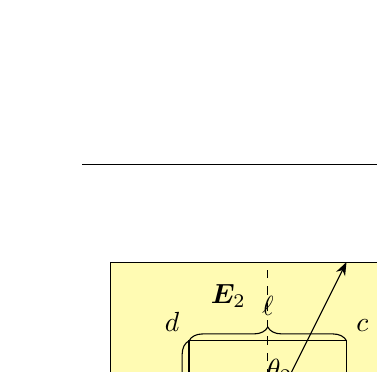
\begin{tikzpicture}[>=Stealth,decoration={brace, amplitude=5}]
              \draw [red](-2,0)--(2,0);
              \draw [fill=green!30](-2,0)--(2,0)--(2,-2)--(-2,-2)--cycle;
              \draw [fill=yellow!30](-2,0)--(2,0)--(2,2)--(-2,2)--cycle;
              \draw [->,black](-2,-2)--(0,0);
              \draw [->,black](0,0)--(1,2);
              \draw (-1,-1)node[below left]{$a$}--(1,-1)node[below right]{$b$}--(1,1)node[above right]{$c$}--(-1,1)node[above left]{$d$}--cycle;
              \draw [decorate](-1,-1)--(-1,1) (-1,0)node[left]{$h$};
              \draw [decorate] (-1,1)--(1,1) (0,1.2)node[above]{$\ell$};
              \draw (1.8,0)node[above]{$\varepsilon_2$};
              \draw (1.8,0)node[below]{$\varepsilon_1$};
              \draw (-0.5,1.3)node[above]{$\vec{E}_2$};
              \draw (0.5,-1.3)node[below]{$\vec{E}_1$};
              \draw [dashed](0,-2)--(0,2);
              \draw (0.2,0.39)arc(60:90:0.39);
              \draw (-0.2,-0.2)arc(-135:-90:0.282);
              \draw (-0.15,-0.25)node[below]{$\theta_1$};
              \draw (0.15,0.35)node[above]{$\theta_2$};
            \end{tikzpicture}
        \end{figure}
        由环路定理,$\oint_L \vec{E}\cdot\dif\vec{l} = \vec{E}_1\cdot \vec{ab}+E_2\cdot \vec{cd} + \delta = 0$
        令$h\to 0\Rightarrow \delta \to 0$,又因为$\vec{ab}=-\vec{cd}$,则$\vec{E}_{t_1}=\vec{E}_{t_2}\Rightarrow \frac{D_{t_1}}{\varepsilon_{r1}} = \frac{D_{t_2}}{\varepsilon_{r2}}$\\
        故电位移矢量的切向分量是不连续的。\\
        法向分量:使用高斯环路定理,运用与上面相似的极限思想,得到$D_{n2}-D_{n1}=\sigma_0$
        \begin{enumerate}[label=(\alph*)]
          \item 若电介质表面无自由电荷(一般情况),则$\sigma_0=0\Rightarrow D_{n1}=D_{n2}\Rightarrow \varepsilon_{r1}E_{n1}=\varepsilon_{r2}E_{n2}$
          \item $\begin{cases}
                  (\vec{D}_2-\vec{D}_1)\cdot\vec{e}_n = \sigma_0\\
                  (\vec{P}_1+\vec{P}_2)\cdot\vec{e}_n = -\sigma'\\
                  \vec{D} = \varepsilon_0 \vec{E}+\vec{P}\\
                  \sigma = \sigma_0+\sigma'
                \end{cases}\Rightarrow (\vec{E}_2-\vec{E}_1)\cdot\vec{e}_n = \frac{\sigma}{\varepsilon_0}$
        \end{enumerate}
        $\vec{D}$和$\vec{E}$在界面上的折射定理:$\frac{\tan\theta_1}{\tan\theta_2} = \frac{D_{t1}}{D_{t2}} = \frac{E_{n{\red 2}}}{E_{n{\red 1}}} = \frac{\varepsilon_{r1}}{\varepsilon_{n2}}$\\
  \item 电势的边值关系:$U_1=U_2$,电势连续
\end{enumerate}

\section{稳恒磁场}
\begin{enumerate}[label=\arabic*.]
    \item $\dif \vec{F}_{12}=I_1 \dif \vec{l}_1 \times  \left(\frac{\mu_0}{4\uppi} \frac{I_2 \dif \vec{l}_2 \times \vec{e}_{12}}{r_{12}^2}\right)=I_1 \dif \vec{l}_1 \times \dif \vec{B}$\quad ({\color{red} 5.3, 6.2, 6.4(考虑F对t的积分)})
    \item 毕萨定律:$\vec{B}=\frac{\mu_0}{4\uppi}\oint_{L}\frac{I\dif \vec{l}\times \vec{e}}{r^2}$
    \item 通电直导线对旁边一点的磁场(通过对直线上的微元积分导出)
          \\ (导线无限长时可以由安培环路定理导出)\quad ({\color{red} 5.8, 8.3(他的计算技巧有点意思)})\\
          \begin{minipage}{0.3\textwidth}
            \begin{tikzpicture}[>=Stealth]
                \draw [->](0,-2.5)--(0,0)node[left]{$I$};
                \draw (0,0)--(0,2.5);
                \fill (2,0)circle(1pt);
                \draw (2,0)node[right]{$P$};
                \draw [dashed](0,-2)--(2,0);
                \draw [dashed](0,2)--(2,0);
                \draw [dashed](0,0)--(1,0)node[above]{$r_0$}--(2,0);
                \draw (0.2,-1.8)arc(45:90:0.3);
                \draw (0.2,1.8)arc(-45:90:0.3);
                \draw (0,-2)node[below right]{$\theta_1$};
                \draw (0,2)node[above right]{$\theta_2$};
            \end{tikzpicture}
          \end{minipage}
          \begin{minipage}{0.65\textwidth}
            $\vec{B}_P=\frac{\mu_0}{4\uppi}\frac{I}{r_0}(\cos \theta_{\red 1} - \cos \theta_{\red 2})$
          \end{minipage}
    \item 左右手定则
    \item 安培环路定理:$\oint_{L}\vec{B}\cdot \dif \vec{l} = \textcolor{red}{\mu_0}\sum I$\quad ({\color{red} 5.10,注意第(1)和(3)穿过圆柱的是$\frac{Ir^2}{a^2}$不是$I$})
    \item 稳恒磁场的基本方程
          \[\text{\color{red}积分形式:}\begin{cases}
            \oiint_{S}\vec{B}\cdot \dif \vec{S} = 0\\
            \oint_{L}\vec{B}\cdot \dif \vec{l} = \textcolor{red}{\mu_0}\sum I
          \end{cases}
            \quad\text{\color{red}微分形式:}
          \begin{cases}
            \nabla \cdot \vec{B} = 0\\
            \nabla \times \vec{B} = \textcolor{red}{\mu_0}\vec{j}
          \end{cases}\]
    \item $I=nqvS$,洛伦兹力:$\vec{F}=q\vec{v}\times \vec{B}$({\red 5.15}螺线管,电子有垂直于磁场和水平速度)
    \item 安培力:磁场对电流的作用($I$线电流,$i$面电流,$j$体电流)\qquad ({\red 5.8})
          \[\begin{cases}
            \vec{F}=\oint I\dif \vec{l}\times \vec{B}\\
            \vec{F}=\iint_S i\dif \vec{S}\times \vec{B}\quad (i=\frac{I}{L}\text{其中L是垂直于I的边长})\\
            \vec{F}=\iiint \vec{j}\dif V\times \vec{B}\quad 
          \end{cases}\]
\end{enumerate}

\section{磁场与物质的相互作用}
\begin{enumerate}[label=\arabic*.]
    \item $\vec{L}=\vec{r}\times \vec{F}=\int \vec{r}\times \dif \vec{F}$
    \item 圆环对中轴上的磁场:\\
          \begin{minipage}{0.5\textwidth}
            \begin{tikzpicture}[>=Stealth]
              \draw (0,0) ellipse [x radius=0.6,y radius=2];%画椭圆 
              \draw (0,0)--(3,0)node[right]{$P$};
              \draw [dashed](3,0)--(4,0);
              \draw [dashed](0,2)--(3,0);
              \draw [dashed](0,-2)--(3,0);
              \draw [->](0,2)--(-0.5,1.9)node[left]{$R$};
              \draw [dashed](0,0)--(0,2)node[above]{$Q$};
              \draw (0,1.8)--(-0.15,1.78)--(-0.15,1.98);
              \draw [->](3,0)--(3.5,0.7)node[right]{$\dif\vec{B}$};
              \draw [->](3,0)--(3.5,-0.7)node[right]{$\dif\vec{B}$};
              \draw (2.8,0.18)--(2.95,0.33)--(3.1,0.2);
              \draw (0,1)node[]{$R$} (2,0)node[]{$r_0$} (2,1.2)node[]{$r$};
              \draw [red](3.6,0)arc(0:52:0.6);
              \draw (3.7,0.2)node[right]{\red $\cos \theta = \frac{R}{R^2+r_0^2}$};
            \end{tikzpicture}
          \end{minipage}
          \begin{minipage}{0.4\textwidth}
            \[\begin{aligned}
              \dif|\vec{B}| &= \frac{\mu_0}{4\uppi}\frac{I\dif \vec{l}_{QR}\times \vec{e}_{PQ}}{r_{PQ}^2}\\
              B &= \oint_{L} \frac{\mu_0}{4\uppi}\frac{I\dif \vec{l}_{QR}\times \vec{e}_{PQ}}{r_{PQ}^2}\cdot {\red \frac{R}{\sqrt{R^2+r_0^2}}}\\
              &= \oint_{L} \frac{\mu_0}{4\uppi}\frac{IR\dif \theta}{R^2+r_0^2}\cdot \frac{R}{\sqrt{R^2+r_0^2}}\\
              &= \frac{\mu_0}{4\uppi}\frac{R^2 I}{(R^2+r_0^2)^{3/2}}\int_{0}^{2\uppi}\dif \theta\\
              &= \frac{\mu_0}{2}\frac{R^2 I}{(R^2+r_0^2)^{3/2}}
            \end{aligned}\]
          \end{minipage}
    \item 电偶极矩(电矩$\vec{p}$)与磁偶极矩(磁矩$\vec{m},\vec{\mu}$)与力矩$\vec{L}$:\quad ({\red 6.6磁矩的定义(一个线圈的磁矩是$\vec{m}=I\vec{S}$,一个圆盘是多个线圈),面电荷与面电流})
          \[\begin{cases}
            \vec{p} = q\vec{l}\\
            \vec{m} = I\vec{S} = IS\vec{e}_n
          \end{cases} \Rightarrow
          \begin{cases}
            \vec{L} = \vec{p}\times \vec{E}\\
            \vec{L} = \vec{m}\times \vec{B}
          \end{cases}
          \]
    \item 磁化强度$\vec{M}=\frac{\sum_i \vec{m}_i}{\Delta V}$
    \item 分子平均磁矩$\vec{m}_a = \frac{\sum_i \vec{m}_i}{n\Delta V} = I_a S_a\Rightarrow \vec{M}=nI_a S_a$
    \item 磁化电流:$\dif I' = I_a n\dif V = nI_a \vec{S}_a\cdot \dif \vec{l}$
    \item 磁通量:$\Phi = \iint \vec{B}\cdot \dif\vec{S}$
    \item 磁化电流:$I'=\iint_S \vec{j'}\cdot \dif \vec{S}\Rightarrow \vec{j'}=\nabla\times\vec{M}$\\
          $I'=\oint \vec{M}\cdot \dif \vec{l}$
    \item 磁介质存在时的高斯定理和环路定理:
          $\vec{B}=\vec{B}_0+\vec{B}'$
          \[\oint_L \vec{B}\cdot \dif \vec{l} = \mu_0 (\sum I_0+\sum I') = \mu_0 (\sum I_0 + \oint_L \vec{M}\cdot\dif\vec{l})\]
          \[\oint \vec{H}\cdot\dif\vec{l}=\sum I_0 \qquad \nabla\times\vec{H}=\vec{j}_0\]
    \item 磁场强度:$\vec{H}=\frac{\vec{B}}{\mu_0}-\vec{M}$,这么看来$\vec{H}$好像是{\red 原磁场}
          \begin{example}
            若螺绕环内充满磁介质,求磁感应强度$B$,已知磁化场的磁感应强度为$B_0$,磁化强度为$M$
          \end{example}
          设螺环半径$R$,总匝数为$N$,则取圆形回路$L$,根据安培环路定理,有:
          \[\oint_L \vec{H}\cdot\dif\vec{l} = 2\uppi RH = \sum I = NI\]
          得\[H = \frac{NI}{2\uppi R} = nI = \frac{\vec{B}}{\mu_0}-\vec{M}\]
          $\because B_0 = \mu_0 nI,\quad \therefore B_0=\mu_0 H$
          $\therefore B = \mu_0 (H+M) = B_0+\mu_0 M$
    \item 螺线管的磁感应强度:$\vec{B}=\mu_0 nI$(注意$n$的量纲$\si{m}^{-1}$)
    \item 磁介质存在时的静磁场:\\
          基本方程:$\begin{cases}
            \oiint \vec{B}\cdot\dif\vec{S} = 0\\
            \oint \vec{H}\cdot\dif\vec{l} = \sum I_0
          \end{cases}$
          本构方程:$\vec{H}=\frac{\vec{B}}{\mu_0}-\vec{M}$
          磁化电流:$\begin{cases}
            \vec{j}'=\nabla\times\vec{M} \\
            \vec{i}'=\vec{M}\times\vec{n}
          \end{cases}$
    \item 磁化系数:$\vec{M}=\chi_m \vec{H}$,$\chi _m$为磁化{\red 率}或磁化{\red 系数},\quad ({\red 6.9(2)})
          \[\vec{B}=\mu_0(\vec{H}+\vec{M})=(\chi _m+1)\mu_0\vec{H}=\mu _r\mu_0\vec{H} = \mu \vec{H}\Rightarrow \vec{M} = \frac{\mu-\mu_0}{\mu_0}\vec{H}\]
          $\mu_{\red r} = 1+\chi_m$是{\red 相对}磁导率,\,$\mu=\mu _r \mu_0$是{\red 介质/绝对}磁导率\quad ({\red 6.11(4),6.12})
    \item 边界条件:\quad ({\red 6.11,6.12})
          \[\begin{cases}
            \oint \vec{H}\cdot\dif\vec{l} = \sum I_{i_0}\\
            \oiint \vec{B}\cdot\dif\vec{S} = 0
          \end{cases}\qquad
          \begin{cases}
            \nabla\times \vec{H} = \vec{j}_0\\
            \nabla\cdot \vec{B} = 0
          \end{cases}
          \]
          介质本构方程:\quad ({\red 6.9(1)})
          \[\vec{B}=\mu_0 \mu _r \vec{H} \qquad \vec{H} = \frac{\vec{B}}{\mu_0}-\vec{M}\]
    \item 磁路定理:\quad ({\red 6.17,6.19,7.9(磁路的等效,注意整条线路都是有磁阻的)})
          \begin{remark}
            注意到$U,\varepsilon,R$的符号和电路一样,但是量纲是完全不同的,只不过遵从一样的公式,气隙相当于磁阻
          \end{remark}
          \begin{enumerate}
            \item 磁位差(电位差):$U_m = Hl = \Phi R_m,\quad \sum H_i l_i = \sum N_j I_j$\quad ($\Phi \leftrightarrow I, R\leftrightarrow R_m$)
            \item 磁动势(电动势):$\varepsilon _m = NI$
            \item 磁阻(电阻):$R_m = \int \frac{\dif l}{\mu S}$
          \end{enumerate}
\end{enumerate}

\section{电磁感应}
\begin{enumerate}[label=\arabic*.]
  \item 动生电动势:$\varepsilon = -\frac{\dif \Phi}{\dif t} = \oint (\vec{v}\times \vec{B})\cdot\dif\vec{l} = BLv$\quad (导体运动造成的磁通量变化)\quad ({\red 7.5,注意(3)的面电荷密度公式$\sigma = \varepsilon_0 E$})
  \item 感生电动势:$\varepsilon = -\frac{\dif \Phi}{\dif t}$\quad (磁场变化造成的磁通量变化)
  \item 非静电力:$\vec{K}=\vec{v}\times \vec{B},\quad \varepsilon = \int \vec{K}\cdot\dif\vec{l} = \int (\vec{v}\times \vec{B})\cdot \dif \vec{l}$\quad (非静电力来源于洛伦兹力)\quad ({\red 7.3})
  \item 全磁通$\Psi = \sum \Phi$
  \item 互感:一个线圈中电流变化时,另一个线圈中产生感应电动势.$\Psi_{21}$是线圈{\red 1}在线圈{\red 2}中的磁链\quad ({\red 7.10(电流到底是从什么方向流进去的?电容公式:$C=\frac{\varepsilon S}{d}$,(3)中$\omega = \frac{1}{\sqrt{LC}}$,7.11磁路转化,注意产生磁动势只有A,线圈匝数不影响磁阻,即不需要乘$N$)})\\
        $\Psi_{21}=M_{21}I_1,\Psi_{12}=M_{12}I_2,M_{12}=M_{21}$
  \item 自感:线圈激发磁场在线圈自身中的磁通.$\Phi = LI\Rightarrow L=\frac{\Phi}{I}$\quad ({\red 7.8,题目漏给了电流$I$,注意磁感应强度$\vec{B}$是需要自己求的,本题极其诡异,7.9})\\
        理想螺线管的自感系数为:$L=\mu_0 n^2 lS = \mu_0 \frac{N^2}{l^2}V=\frac{\mu_0 N^2 S}{l}$(推导见{\red 7.14})
  \item 自感与互感的关系:$M_{12}=M_{21}=\sqrt{L_1 L_2}$
  \item 通电长直导线和旁边一圆环的互感:
        \[\begin{aligned}
          \Psi &= \iint_S \vec{B}\cdot \dif \vec{S}=\frac{\mu_0 I}{2\uppi}\int_{0}^{R}\dif \rho \int_{0}^{2\uppi}\frac{\rho \dif \rho \dif \theta}{d+\rho \cos \theta}\\
          &= \frac{\mu_0 I}{\uppi}\int_{0}^{R}\rho \dif \rho \int_{0}^{\uppi}\frac{\dif \theta}{d+\rho \cos \theta}\\
          &= \frac{\mu_0 I}{\uppi}\int_{0}^{R}\rho \dif \rho \frac{2}{\sqrt{d^2-\rho ^2}}\left(\sqrt{\frac{d-\rho}{d+\rho}\tan \frac{\theta}{2}}\right)\Big|_{0}^{\uppi}\\
          &= \mu_0 I\int_{0}^{R} \frac{\rho \dif \rho}{\sqrt{d^2-\rho ^2}}\\
          &= \mu_0 I(d-\sqrt{d^2-R^2})\\
          M &= \mu_0(d-\sqrt{d^2-R^2})
        \end{aligned}\]
  \item 此处应有涡旋电场,但是习题好像没有,就不写了
  \item 各种暂态方程:\quad ({\red 7.16,8.1})
        \begin{enumerate}[label=(\alph*)]
          \item RL电路:$I=\frac{\varepsilon}{R}(1-\e^{-\frac{R}{L}t})$,可令$I_0=\frac{\varepsilon}{R},\tau=\frac{L}{R}$,这样形式好看点
          \item RC电路:$q=q_0(1-\e^{-\frac{t}{\tau}}),\quad \tau=RC$
          \item RCL电路:$q=q_0-q_0\e^{-\beta t}(\cos \omega t +\frac{\beta}{\omega}\sin \omega t)\quad \beta=\frac{R}{2L},\omega_0=\frac{1}{\sqrt{LC}},q_0=C\varepsilon $
        \end{enumerate}
  \item 磁能:$W=\frac{LI^2}{2}=\frac{CU^2}{2}=\frac{1}{2}L_1 I_1^2+\frac{1}{2}L_2 I_2^2+MI_1 I_2$\quad ({\red 8.1})
  \item 互感磁能(相互作用能):$W_{12}=M_{21}I_1 I_2 = \Phi_{21}I_2$\quad ({\red 8.2,别忘了安培环路求$\vec{B}$,8.5(此处$a<r<b$仍为空心,$r<a$处为实心圆柱体)})
  \item 磁能密度:$w = \frac{W}{V}=\frac{1}{2}BH=\frac{1}{2}\vec{B}\cdot \vec{H}$\quad ({\red 8.2,此处磁能密度运用了$w=\frac{1}{2}\vec{B}\cdot \vec{H}=\frac{1}{2}B \frac{B}{\mu_0}=\frac{B^2}{2\mu_0}$,B和H的关系别忘了})
\end{enumerate}

\section{Maxwell方程组}
\begin{enumerate}[label=(\arabic*)]
  \item 静电学的实验规律:库仑定律$\vec{F}=\frac{1}{4\uppi \varepsilon_0}\frac{q_1 q_2}{r^3}\vec{e}_r$\\
        由库仑定律和电场叠加原理得到描述静电场的高斯定理和环路定理:\[\oiint _S \vec{D}\cdot \dif \vec{S}=\sum q_i,\qquad \oint_L \vec{E}\cdot \dif \vec{l} = 0\]
  \item 静磁学的实验规律:安培定律$\vec{F}_{12} = \frac{\mu_0}{4\uppi}\cdot \frac{I_2\dif \vec{l}_2\times (I_1 \dif \vec{l}_1\times \vec{e}_r)}{r^3}$\\
        由安培定律和场强叠加原理得到描述静磁场的高斯定理和安培环路定理:\[\oiint \vec{B}\cdot \dif \vec{S} = 0,\qquad \oint_L \vec{H}\cdot \dif \vec{l} = \sum I_i\]
  \item 麦克斯韦提出了法拉第电磁感应定律的物理本质是{\red 随时间变化的磁场在其周围激发涡旋电场},即:
        \[\oint_L \vec{E}_{\text{旋}}\cdot \dif \vec{l} = -\iint \frac{\partial \vec{B}}{\partial t}\cdot \dif \vec{S},\qquad \nabla \times  \vec{E}_{\text{旋}} = -\frac{\partial \vec{B}}{\partial t}\]
  \item 电荷守恒定律(实验总结):\[\oiint_S \vec{j}\cdot \dif \vec{S} = -\frac{\dif}{\dif t}\iiint_{V}\rho \dif V = -\iiint_V \frac{\partial \rho}{\partial t}\dif V,\qquad \nabla \cdot \vec{j} + \frac{\partial \rho}{\partial t} = 0\]
  \item 实验规律的推广:
        \begin{enumerate}[label=(\roman*)]
          \item 静电场环路积分的推广:\[\oint_L \vec{E}\cdot \dif \vec{l} = \oint_L \vec{E}_{\text{势}}\cdot\dif\vec{l}+ \oint_L \vec{E}_{\text{旋}}\cdot\dif\vec{l} = -\iint_S \frac{\partial \vec{B}}{\partial t}\cdot \dif \vec{S}\Rightarrow \nabla\times \vec{E} = -\frac{\partial \vec{B}}{\partial t}\]
          \item 静电场高斯定理的推广:\[\oiint_S \vec{E}\cdot \dif \vec{S} = \oiint_S (\vec{E}_{\text{势}}+\vec{E}_{\text{旋}})\cdot \dif \vec{S} = \frac{1}{\varepsilon_0}\sum q_i\Rightarrow \oiint_S \vec{D}\cdot \dif \vec{S} = \sum q_i\Rightarrow \nabla \cdot \vec{D} = \rho_0\]
          \item 静磁场高斯定理的推广:$\nabla\cdot\vec{B}\equiv\const$(PPT上的推导我也没有看懂,写个结论得了)
          \item 安培环路定理的推广:\[\oint_L \vec{H}\cdot \dif \vec{l} = \sum I = \iint_S \vec{j}\cdot \dif \vec{S} = \iint_S (\vec{j}_0 + \frac{\partial \vec{D}}{\partial t})\cdot \dif \vec{S} = 0\Rightarrow \nabla\times \vec{H} = \vec{j}_0 + \frac{\partial \vec{D}}{\partial t}\]
          \item $I_d = \frac{\dif \Phi _D}{\dif t}$定义为{\red 位移电流$I_d$,注意此处的$\Phi_D = \iint_S \vec{D}\cdot \dif \vec{S}$是{\blue 电位移通量}不是{\blue 磁通量}},\\
                {\blue 电位移矢量的时间变化率}定义为{\red 位移电流密度$j_d$},传导电流(即漏电流,电路电流)和位移电流合起来称为{\red 全电流$I$}\\
                ({\red 10.1(1)$I_d = \frac{\dif \Phi}{\dif t} = S\cdot \frac{\partial \vec{D}}{\partial t} = \varepsilon S \frac{\partial \vec{E}}{\partial t} = \frac{\varepsilon S}{d}\cdot \frac{\dif V}{\dif t} = C \frac{\dif V}{\dif t}$(2)漏电流就是电路电流$I = \frac{V}{R}$,
                \quad 10.2(1)位移电流和传导电流和角频率和电导率的关系,\quad 10.3(电位移矢量$\vec{D}$和面电荷密度$\sigma$)})
                \begin{corollary}
                  \mbox{}\\
                  位移电流密度$\vec{j}_d = \frac{I_d}{S} = \varepsilon_0 \frac{\partial \vec{E}}{\partial t} = \frac{\partial \vec{D}}{\partial t}$\\
                  $j_0=\sigma E\Rightarrow E=\rho j_0$($\sigma$是电导率)
                \end{corollary}
          \item 位移电流的本质:随时间变化的电场可以激发磁场
        \end{enumerate}
  \item \[\begin{cases}
          \oint_L \vec{E}\cdot \dif \vec{l} = -\iint \frac{\partial \vec{B}}{\partial t}\cdot \dif \vec{S}\\
          \oint_L \vec{H}\cdot \dif \vec{l} = \sum I_0 + \iint_S \frac{\partial \vec{D}}{\partial t}\cdot \dif \vec{S}
        \end{cases}\qquad
        \begin{cases}
          \nabla \cdot \vec{D} = \rho_0\\
          \nabla \times \vec{E} = -\frac{\partial \vec{B}}{\partial t}\\
          \nabla\cdot \vec{B} = 0\\
          \nabla\times \vec{H} = \vec{j}_0 + \frac{\partial \vec{D}}{\partial t}
        \end{cases}
        \]
        题目:PPT8.1.31,
  \item Maxwell方程组的边界条件({\red 10.4})
        \begin{itemize}
          \item $\vec{n}\cdot (\vec{D}_2-\vec{D}_1)=\sigma_0$
          \item $\vec{n}\times (\vec{E}_2-\vec{E}_1)=0$
          \item $\vec{n}\cdot (\vec{B}_2-\vec{B}_1)=0$
          \item $\vec{n}\times (\vec{H}_2-\vec{H}_1)=i_0$
        \end{itemize}
  \item $\sqrt{\varepsilon}E_0=\sqrt{\mu}H_0$
  \item 电磁波的传播速度:$v=\frac{\omega}{k}=\frac{c}{\sqrt{\varepsilon_r \mu_r}}=\frac{v}{\sqrt{\varepsilon \varepsilon_0 \mu \mu_0}}=\frac{c}{n}=\lambda f$
  \item 能流密度(Poynting矢量)$\vec{S}\equiv \vec{E}\times \vec{H}$
  \item 动量密度$\vec{g}=\vec{D}\times \vec{B}$
  \item 能量密度$\omega \equiv \frac{1}{2}\left(\varepsilon E^2+\frac{1}{\mu}B^2\right)$
\end{enumerate}

\section{定义式总结区}
\begin{itemize}
  \item $\vec{B}=\frac{1}{4\uppi}\oint_L \frac{I\dif \vec{l}\times \vec{e}}{r^2}=\mu_0 nI=\mu_0 H=\mu_0(H+M)=\mu n_0 I=\mu_0 \frac{N}{l}I({\color{red}\text{螺线管}})$\\
        无限长通电直导线周围$r_0$处的磁场:安培环路定理推得$B=\frac{\mu_0 I}{2\uppi r}$\\
        那么非无限长则除去$2=\cos 0-\cos \uppi$得到$B=\frac{\mu_0 I}{4\uppi r_0}(\cos \theta_1-\cos \theta_2)$\\
        半径为$R$的圆环轴线上$r_0$处的磁场,量纲应该相同,且圆环应该乘以$2\uppi$那么最后大约得到$B=\frac{\mu_0 I}{2}\frac{R^2}{(R^2+r_0^2)^{\frac{3}{2}}}$
  \item \[\begin{aligned}
          \vec{F} &= I\vec{l}\times\vec{B} = q\vec{v}\times\vec{B}\\
          &= \oint_L I\dif\vec{l}\times\vec{B}\\
          &= \iint_S i\cdot\dif\vec{S}\times\vec{B}\\
          &= \iint_V \vec{j}\dif V\vec{B}\\
        \end{aligned}\]
  \item Lorentz力$\vec{F}=q(\vec{E}+v\times \vec{B})$
  \item $I=nqvS$
  \item 磁矩$\vec{m}=I\vec{S}=IS\vec{e_n}, \vec{L}=\vec{m}\times\vec{B}$(一个圆环电流$I$,$\vec{S}$是该圆环面积)
  \item 磁通量$\Phi=\iint \vec{B}\cdot \dif \vec{S} = LI = MI$
  \item 磁化电流$I'=\oint \vec{M}\cdot \dif \vec{l}$
  \item 磁场强度$\vec{H}=\frac{\vec{B}}{\mu_0}-\vec{M}$
  \item 磁化系数$\vec{M}=\chi_m \vec{H}$
  \item 磁位差$U_m=H\ell=NI=\Phi R_m$
  \item 磁动势$\varepsilon_m = NI$
  \item 磁阻$R_m=\int \frac{\dif l}{\mu S}$
  \item 电动势$\varepsilon=-\frac{\dif \Phi}{\dif t}=\oint (\vec{v}\times \vec{B})\cdot \dif \vec{L} =BLv = \int \vec{K}\cdot\dif\vec{l}$
  \item 非静电力$\vec{K}=\vec{v}\times \vec{B}$
  \item 自感系数$L=\frac{\Phi}{I}=\mu_0 n^2 \ell S = \mu_0 \frac{N^2}{l^2}V = \frac{\mu_0 N^2 S}{l}$
  \item 自感与互感$M_{12}=\sqrt{L_1 L_2}$
  \item 磁能$W=\frac{LI^2}{2}=\frac{CU^2}{2}=\frac{1}{2}L_1 I_1^2 +\frac{1}{2}L_2 I_2^2 +MI_1I_2$
  \item 互感磁能(相互作用能)$W_{12}=M_{21}I_1I_2=\Phi_{21}I_2$
  \item 磁能密度$w=\frac{W}{V}=\frac{1}{2}BH=\frac{B^2}{2\mu_0}$
  \item 位移电流$I_d=\frac{\dif \Phi _D}{\dif t}=\frac{\dif}{\dif t}\iint_S \vec{D}\cdot \dif \vec{S}$\\
        位移电流密度$j_d=\frac{I_d}{S}=\varepsilon_0 \frac{\partial \vec{E}}{\partial t}=\frac{\partial \vec{D}}{\partial t}$
        传导电流密度$j_0=\sigma E$
  \item Maxwell方程组:
        \[\begin{aligned}
          \oint_L \vec{E}\cdot \dif \vec{\ell} &= -\iint \frac{\partial \vec{B}}{\partial t}\dif \vec{S} &\Rightarrow \nabla\times \vec{E} &= -\frac{\partial \vec{B}}{\partial t}\\
          \oint_L \vec{H}\cdot \dif \vec{\ell} &= \iint \left(\vec{j}_0+\frac{\partial \vec{D}}{\partial t}\right)\cdot \dif \vec{S} &\Rightarrow \nabla\times \vec{H} &= \vec{j}_0+\frac{\partial \vec{D}}{\partial t}
        \end{aligned}\]
  \item $j_0=\sigma E$
  \item 能量密度$\omega=\frac{1}{2}(\vec{D}\times \vec{E}+\vec{B}\times \vec{H})$
  \item 能流密度(玻印廷矢量)$\vec{S}= \vec{E}\times \vec{H}$
  \item 动量密度$\vec{g}=\vec{D}\times \vec{B}$
\end{itemize}

\appendix
\section{物理量}
\begin{table}[H]
  \centering
  \renewcommand\arraystretch{1.5}
  \begin{tabular}{cccc}
    \toprule
    物理量 & 英文 & 符号 & 单位 \\
    \midrule
    磁感应强度 & magnetic f{}lux density & $\vec{B}$ & T($\si{NA^{-1}m^{-1}}$)\\
    磁通量 & magnetic f{}lux & $\Phi$ & Wb($\si{V\cdot s}$) \\
    磁偶极矩(磁矩) & magnetic dipole moment & $\vec{m},\vec{\mu}$ & $\si{A\cdot m^2}$ \\
    磁{\red 化}强度 & magnetization & $\vec{M}$ & A/m \\
    磁{\red 场}强度 & magnetic f{}ield intensity & $\vec{H}$ & A/m \\
    磁位差 & magnetic potential & $U_m$ & A \\
    磁动势 & magnetic potential energy & $\varepsilon _m$ & A \\
    磁阻 & magnetic resistance & $R_m$ & $\si{H^{-1}}$ \\
    全磁通 & total magnetic f{}lux & $\Psi$ & Wb \\
    \bottomrule
  \end{tabular}
\end{table}
\begin{remark}
  \begin{enumerate}[label=(\alph*)]
    \item 磁场强度$\vec{H}$类似电位移矢量$\vec{D}$
  \end{enumerate}
\end{remark}
常数$\mu_0 = 4\uppi\times 10^{-7}$

\section{存疑的地方}
\begin{enumerate}[label=(\roman*)]
  \item 螺线管到底咋绕的,通电螺绕环,矩形螺线管,圆形螺线管
  \item 圆柱面,电流沿柱面而非圆周方向流动,此时的中心轴线磁场方向如何确定({\red 8.2})
  \item 电位移矢量$\vec{D}$,面电荷密度$\sigma$,电导率$\sigma$的关系
\end{enumerate}

\end{document}